\chapter{Experiments and Results}
\label{cha:experiments}

\section{Experimental Setup}
\label{sec:experimental-setup}

\begin{comment}
Trying and failing is a major part of research. However, to have a chance of success you need a plan driving the experimental research, just as you need a plan for your literature search. Further, plans are made to be revised and this revision ensures that any further decisions made are in line with the work already completed.

The plan should include what experiments or series of experiments are planned and what questions the individual or set of experiments aim to answer. Such questions should be connected to your research questions, so that in the evaluation of your results you can discuss the results wrt to the research questions.
\end{comment}

\begin{comment}
The experimental setup should include all data --- parameters, etc. --- that would allow a person to repeat your experiments.
This will thus be the actual instantiation for each experiment of the general architecture described in Chapter~\ref{cha:architecture}.
\end{comment}

The experiments conducted to evaluate the performance of GeoGPT on geospatial tasks are divided into three main approaches, as elaborated upon in

\subsection{Quantitative Approach: Benchmarking}

The first approach seeks to evaluate its ability to successfully answer questions that have a concrete answer. To do this, a Q\&A dataset was constructed. This dataset consists of geospatial questions with corresponding correct answers. For each sample of the dataset, a description of how a human would find it natural to approach the problem. This description is provided  as step-by-step path towards the solution, and is only included to guide any reader of this thesis as to how the system would be expected to solve the system. Only the questions and their answers are used in the actual evaluation. The full Q\&A dataset can be found in \autoref{app:qa-for-benchmark}. This set of experiments will allow for quantitative assessment of GeoGPT's GIS-abilities, and is a feasible way of benchmarking the system.

\subsection{Qualitative Approach: Case Studies}

The second set of experiments are constructed to evaluate GeoGPT's ability to answer analytical questions that may have different answers. For these experiments the main focus was to see how it reasons about the task, and how it makes use of the available data to provide the user with useful insights that can be drawn from the data. Unlike the above-mentioned benchmarking approach, this set of experiments will consist of a few case studies that are evaluated qualitatively through discussion.

\subsection{Consistency Analysis: Investigating Repeatability}

The third and final approach will focus on the consistency of the system, its ability to repeatedly provide an acceptable answer to the same user question. Additionally, this set of experiments will investigate to what extent the experience of the prompter --- the human user --- affects GeoGPT's ability to provide consistent results.

\section{Experimental Results}
\label{sec:experimental-results}

It is worth noting that two slightly different models were used during testing. The explanation of this is the release of the \texttt{gpt-4-turbo-2024-04-09} in mid-April. According to OpenAI, \enquote{this new model is better at math, logical reasoning, and coding} compared to \texttt{gpt-4-0125-preview}\footnote{OpenAI has a Github repository containing the code they use to evaluate their \glspl{acr:llm} and benchmark results for OpenAI models and reference models from other companies: \url{https://github.com/openai/simple-evals}.}, which is the model that was used at the start of the experimentation phase of the master's thesis. At the new model's release, a decision was made to use this for the remaining experiments. The experiments that had already been conducted were not re-run due to time constraints and a belief that these slight model upgrades would not significantly change the outcome of the experiments.

\begin{comment}
Results should be clearly displayed and should provide a suitable representation of your results for the points you wish to make.
Graphs should be labelled in a legible font. If more than one result is displayed in the same graph, then these should be clearly marked.
Please choose carefully rather than presenting every result. Too much information is hard to read and often hides the key information you wish to present. Make use of statistical methods when presenting results, where possible to strengthen the results.
Further, the format of the presentation of results should be chosen based on what issues in the results you wish to highlight.
You may wish to present a subset in the experimental section and provide additional results in an appendix.
Point out specifics here but save the overall/general discussion to the Discussion chapter.
\end{comment}

\subsection{Quantitative Results}

\begin{figure}[htbp]
    \centering
    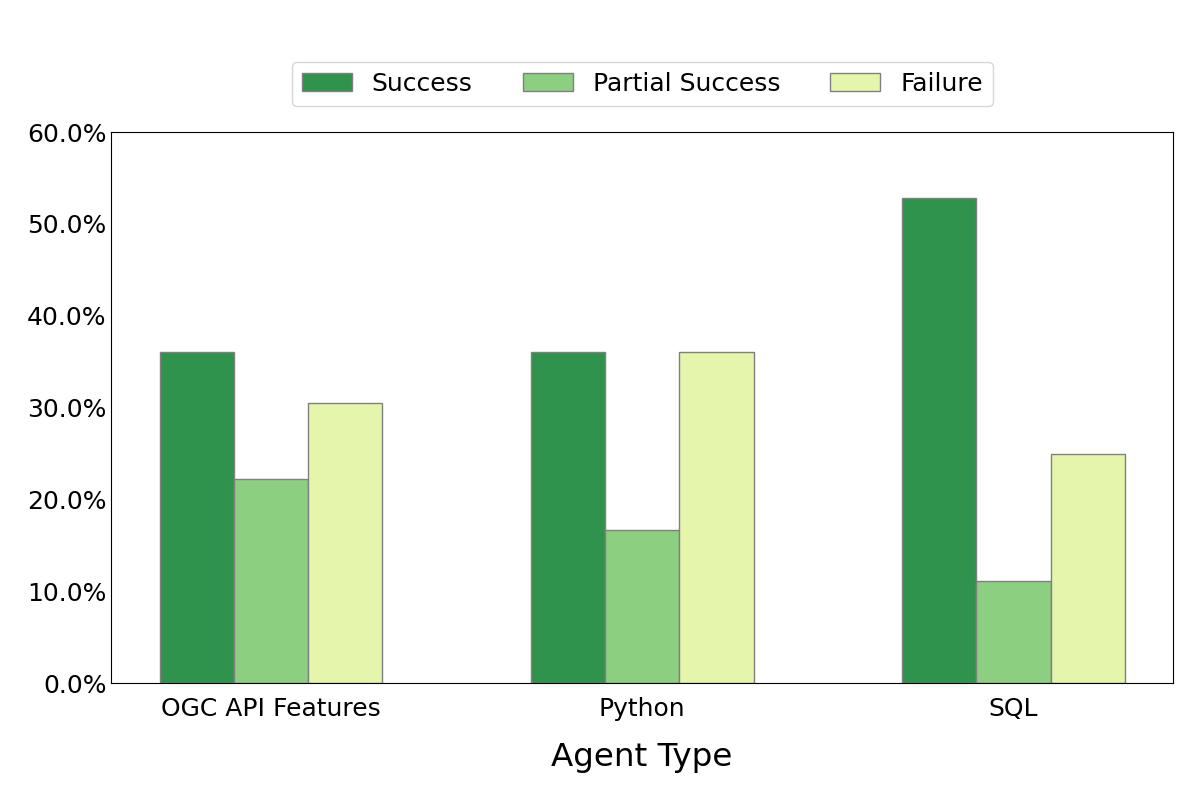
\includegraphics[width=\textwidth]{outcome_distribution_bar_chart.png}
    \caption{Outcome Distribution}
    \label{fig:outcome_distribution}
\end{figure}

\begin{figure}[htbp]
    \centering
    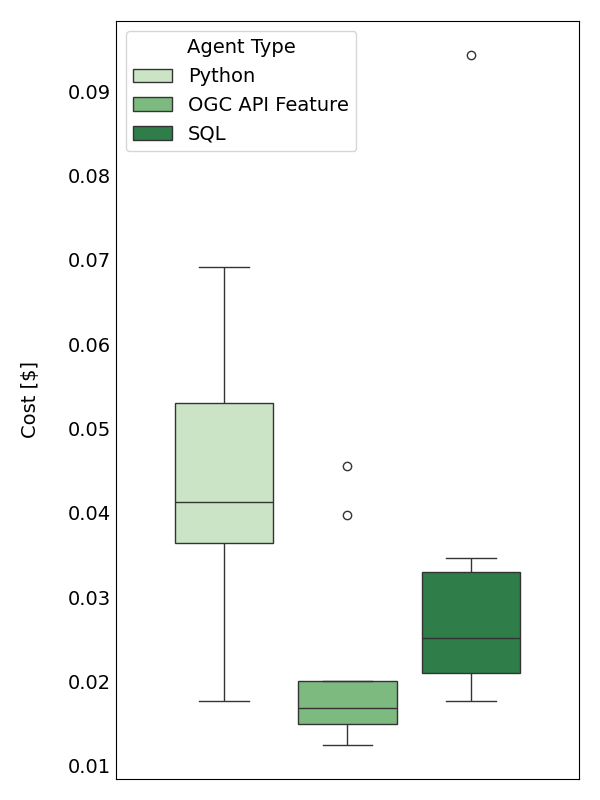
\includegraphics[width=0.8\textwidth]{cost_box_plot.png}
    \caption{Cost per Agent Type}
    \label{fig:cost_box_plot}
\end{figure}

\begin{figure}[htbp]
    \centering
    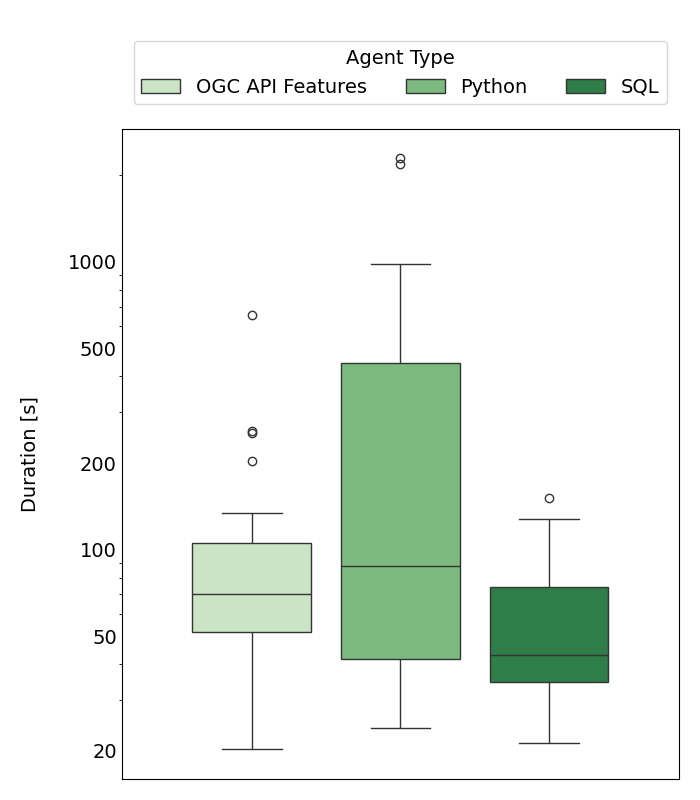
\includegraphics[width=0.8\textwidth]{duration_box_plot.png}
    \caption{Duration per Agent Type}
    \label{fig:duration_box_plot}
\end{figure}

